\clearpage
\section{Corrected transfer uncertainty and historical record}
\label{app:derived-transfer}

The scientific revision retains the original prediction ledger and its historical numerical derivations while introducing an additive corrected target projection. The correction changes both target values and eligibility; current statistics use all \AuditTransferCount{} eligible Extended-new queries derived from the 508 registered candidates. Historical46 is unaffected by the low/medium correction. \evidence{GT01}

\begingroup\scriptsize\setlength{\tabcolsep}{3pt}
\begin{longtable}{lrrr}
\caption{All 508 extended candidates retained. Nearest TTC within 50 ms inclusive, earlier ties; corrected labels yield 460 eligible queries. Historical46 retains all 46 and is scored separately.}\label{tab:audit-transfer-eligibility}\\
\toprule
Sequence & Candidates & Historical eligible & Corrected eligible \\
\midrule
CCRm-low-0-overlap-0 & 16 & 16 & 16 \\
CCRm-low-100-overlap-100 & 16 & 13 & 13 \\
CCRm-low-50-overlap-50 & 16 & 15 & 15 \\
CCRm-medium-0-overlap-0 & 16 & 13 & 13 \\
CCRm-medium-100-overlap-100 & 16 & 14 & 14 \\
CCRm-medium-50-overlap-50 & 16 & 15 & 15 \\
CCRs-1-high-0-overlap-0 & 16 & 15 & 15 \\
CCRs-1-high-100-overlap-100 & 16 & 15 & 15 \\
CCRs-1-high-50-overlap-50 & 16 & 15 & 15 \\
CCRs-1-low-0-overlap-0 & 16 & 13 & 13 \\
CCRs-1-low-100-overlap-100 & 16 & 15 & 10 \\
CCRs-1-low-50-overlap-50 & 16 & 16 & 16 \\
CCRs-1-medium-0-overlap-0 & 16 & 14 & 14 \\
CCRs-1-medium-100-overlap-100 & 16 & 15 & 12 \\
CCRs-1-medium-50-overlap-50 & 16 & 15 & 15 \\
CCRs-2-high-100-overlap-100 & 12 & 11 & 11 \\
CCRs-2-low-100-overlap-100 & 16 & 16 & 16 \\
CCRs-2-medium-100-overlap-100 & 16 & 15 & 15 \\
CCRs-3-low-100-overlap-100 & 16 & 13 & 13 \\
CCRs-3-medium-100-overlap-100 & 16 & 16 & 16 \\
CCRs-side-high & 16 & 16 & 16 \\
CCRs-side-low & 16 & 16 & 16 \\
CCRs-side-medium & 16 & 16 & 16 \\
CPLA-high & 16 & 15 & 15 \\
CPLA-low & 16 & 15 & 15 \\
CPLA-medium & 16 & 15 & 15 \\
CPNA-high & 16 & 15 & 15 \\
CPNA-low & 16 & 12 & 12 \\
CPNA-medium & 16 & 13 & 13 \\
CPNAO-high & 16 & 14 & 14 \\
CPNAO-low & 16 & 16 & 16 \\
CPNAO-medium & 16 & 15 & 15 \\
\bottomrule
\end{longtable}
\endgroup


\subsection{Target reassociation versus metric recomputation}
The source audit first reproduces every historical target or exclusion for all 554 saved candidates under the old source assignment. It then replaces only the two verified low/medium curves and applies the unchanged nearest-label rule at the unchanged native timestamps. The projection records the corrected source SHA-256, target time, time distance, and before/after label neighbors. The separate metric builder verifies the projection hash, all prediction fields against the historical CSV, and the nearest-neighbor decisions before recomputing statistics.

This provides distinct checks of recording/source identity and arithmetic. The original raw sensor streams are not needed for saved-prediction scoring. Repeating the full association audit additionally requires the source curves and original query manifest pinned in \path{audit_20261104/transfer_reassociation.json}; no target-driven clock fitting is involved.

\subsection{Paired complete-sequence bootstrap}
Each of 10,000 resamples draws 32 sequence-group identities with replacement and includes all eligible queries from each selected group, repeating queries when their group is drawn more than once. PHASE-TTC and RGB share the draw. Pooled mean, median, and p95 differences use NumPy's linear quantiles with seed 20261028. The three intervals contain zero (Table~\ref{tab:audit-transfer-bootstrap}). They condition on the saved models and historically exposed recordings.

The mean difference is \AuditMeanDelta{}\,s, median difference \AuditMedianDelta{}\,s, and p95 difference \AuditPninetyfiveDelta{}\,s. Complete-precision estimates and intervals reside in \path{audit_20261104/corrected_transfer_statistics.json}. Sequence-macro MAE/RTE comparisons against Garl use their original 2,000 group resamples and seed 7; they are separate estimands from the pooled PHASE--RGB comparison.

\subsection{Sequence-level comparisons}
\begin{figure}[H]
\centering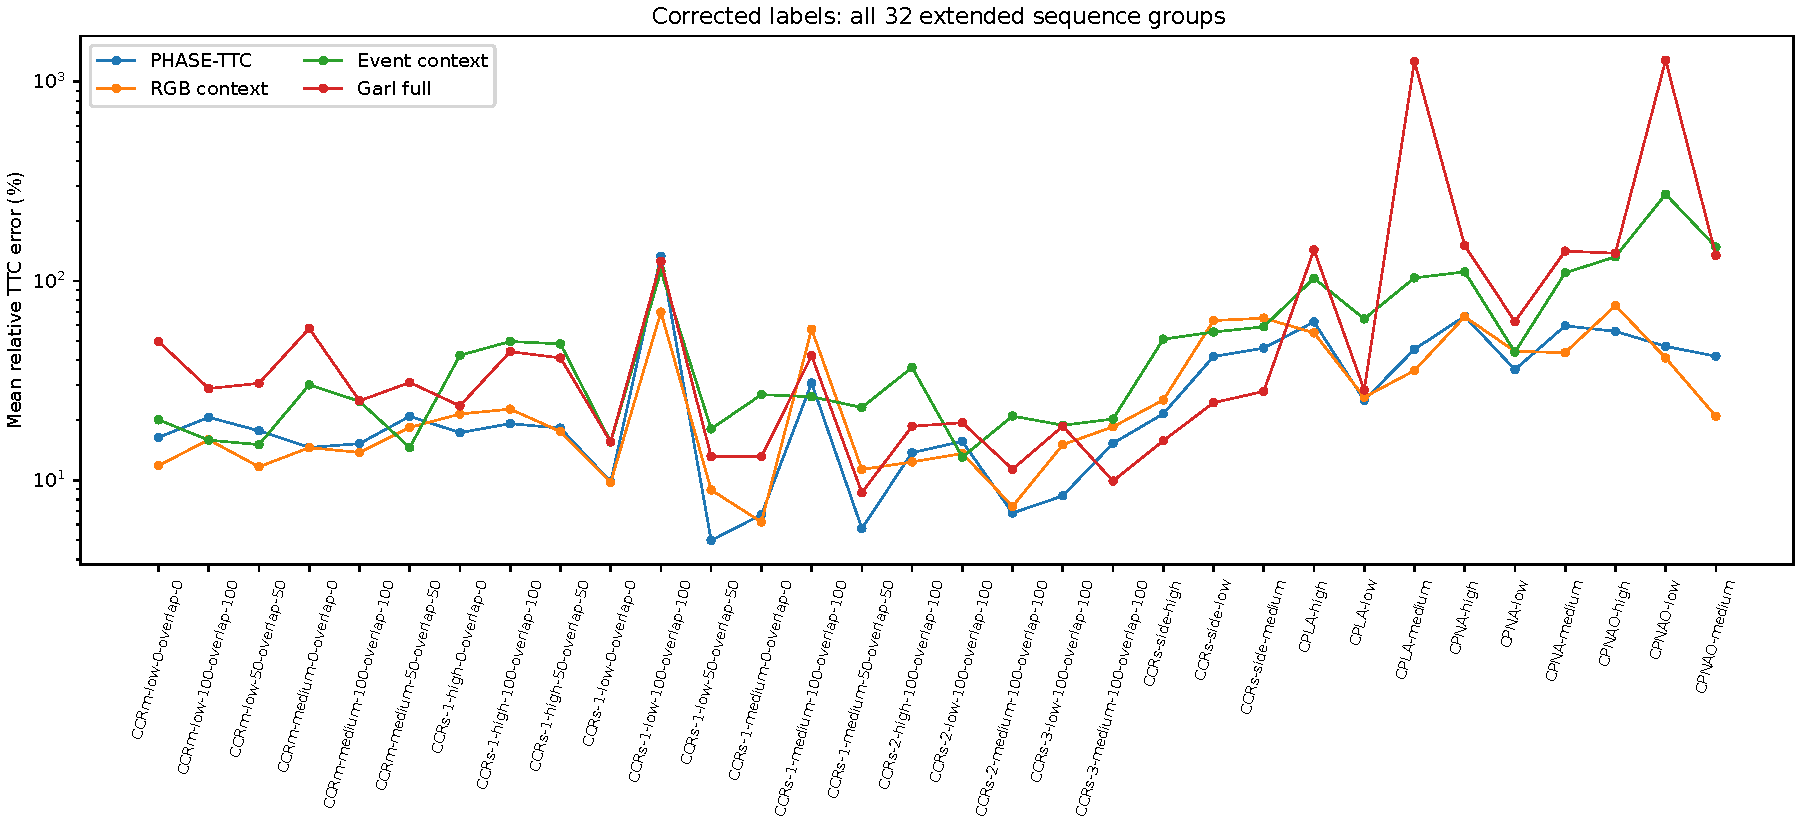
\includegraphics[width=\linewidth,height=.70\textheight,keepaspectratio]{figures/audit_transfer_sequences.pdf}
\caption{\textbf{Corrected sequence-level relative errors.} Curves show each model's mean relative TTC error on a logarithmic scale; lower is better. The thirty-two sequence groups retain their native identities. Table~\ref{tab:audit-transfer-sequences} gives the corrected eligible query counts and errors.}
\label{fig:transfer-sequence}
\end{figure}
\FloatBarrier
{\small\begingroup\scriptsize\setlength{\tabcolsep}{3pt}
\begin{longtable}{lrrrrrrrrr}
\caption{Corrected extended-cohort errors by all 32 sequence groups. MAE in seconds; RTE in percent.}\label{tab:audit-transfer-sequences}\\
\toprule
Sequence & $n$ & PHASE MAE & RTE & RGB MAE & RTE & Event MAE & RTE & Garl MAE & RTE \\
\midrule
CCRm-low-0-overlap-0 & 16 & 0.535 & 16.401 & 0.350 & 11.845 & 0.548 & 20.089 & 1.143 & 49.694 \\
CCRm-low-100-overlap-100 & 13 & 1.241 & 20.687 & 0.976 & 15.960 & 1.056 & 15.888 & 1.607 & 28.848 \\
CCRm-low-50-overlap-50 & 15 & 0.873 & 17.699 & 0.563 & 11.675 & 0.846 & 15.084 & 1.483 & 30.650 \\
CCRm-medium-0-overlap-0 & 13 & 1.183 & 14.607 & 1.097 & 14.565 & 1.707 & 30.105 & 4.746 & 57.778 \\
CCRm-medium-100-overlap-100 & 14 & 1.308 & 15.253 & 1.225 & 13.787 & 1.800 & 24.898 & 2.020 & 25.036 \\
CCRm-medium-50-overlap-50 & 15 & 1.632 & 20.935 & 1.495 & 18.408 & 1.457 & 14.583 & 2.412 & 30.928 \\
CCRs-1-high-0-overlap-0 & 15 & 0.581 & 17.324 & 0.691 & 21.492 & 1.246 & 42.358 & 0.715 & 23.613 \\
CCRs-1-high-100-overlap-100 & 15 & 0.436 & 19.227 & 0.473 & 22.748 & 1.033 & 49.698 & 1.005 & 44.193 \\
CCRs-1-high-50-overlap-50 & 15 & 0.495 & 18.253 & 0.441 & 17.546 & 1.337 & 48.337 & 0.992 & 41.092 \\
CCRs-1-low-0-overlap-0 & 13 & 0.457 & 9.808 & 0.364 & 9.735 & 0.539 & 15.563 & 0.622 & 15.576 \\
CCRs-1-low-100-overlap-100 & 10 & 1.882 & 133.204 & 1.144 & 69.806 & 2.124 & 112.589 & 2.062 & 125.459 \\
CCRs-1-low-50-overlap-50 & 16 & 0.107 & 4.983 & 0.217 & 8.934 & 0.348 & 18.090 & 0.379 & 13.154 \\
CCRs-1-medium-0-overlap-0 & 14 & 0.177 & 6.715 & 0.157 & 6.170 & 0.638 & 26.896 & 0.353 & 13.138 \\
CCRs-1-medium-100-overlap-100 & 12 & 1.165 & 30.732 & 1.915 & 57.257 & 1.106 & 26.229 & 1.256 & 42.152 \\
CCRs-1-medium-50-overlap-50 & 15 & 0.102 & 5.726 & 0.202 & 11.323 & 0.447 & 23.179 & 0.206 & 8.664 \\
CCRs-2-high-100-overlap-100 & 11 & 0.443 & 13.747 & 0.400 & 12.346 & 1.185 & 36.812 & 0.588 & 18.652 \\
CCRs-2-low-100-overlap-100 & 16 & 0.979 & 15.666 & 0.802 & 13.616 & 0.869 & 13.056 & 1.091 & 19.437 \\
CCRs-2-medium-100-overlap-100 & 15 & 0.164 & 6.839 & 0.177 & 7.389 & 0.501 & 20.995 & 0.290 & 11.356 \\
CCRs-3-low-100-overlap-100 & 13 & 0.359 & 8.348 & 0.595 & 15.077 & 0.779 & 18.878 & 0.876 & 18.667 \\
CCRs-3-medium-100-overlap-100 & 16 & 0.531 & 15.324 & 0.629 & 18.539 & 0.598 & 20.285 & 0.294 & 9.908 \\
CCRs-side-high & 16 & 0.466 & 21.539 & 0.570 & 25.262 & 1.010 & 51.047 & 0.334 & 15.771 \\
CCRs-side-low & 16 & 1.207 & 41.760 & 2.146 & 63.283 & 1.460 & 55.465 & 1.104 & 24.485 \\
CCRs-side-medium & 16 & 1.507 & 46.059 & 1.889 & 65.107 & 1.893 & 58.878 & 1.611 & 27.916 \\
CPLA-high & 15 & 1.051 & 62.285 & 0.908 & 54.915 & 1.723 & 103.255 & 2.274 & 143.221 \\
CPLA-low & 15 & 0.775 & 25.190 & 0.949 & 26.090 & 1.829 & 64.513 & 0.704 & 28.375 \\
CPLA-medium & 15 & 0.731 & 45.430 & 0.622 & 35.531 & 1.796 & 103.663 & 15.406 & 1265.982 \\
CPNA-high & 15 & 1.038 & 66.503 & 1.072 & 66.142 & 1.543 & 111.085 & 2.122 & 150.708 \\
CPNA-low & 12 & 1.133 & 35.904 & 1.467 & 44.345 & 1.275 & 43.942 & 2.334 & 62.536 \\
CPNA-medium & 13 & 0.924 & 59.614 & 0.712 & 43.684 & 1.669 & 109.875 & 2.212 & 141.205 \\
CPNAO-high & 14 & 1.432 & 55.864 & 2.038 & 75.177 & 3.032 & 132.298 & 3.517 & 137.892 \\
CPNAO-low & 16 & 1.035 & 46.955 & 0.956 & 41.095 & 4.935 & 272.685 & 39.943 & 1283.264 \\
CPNAO-medium & 15 & 0.511 & 41.916 & 0.248 & 20.936 & 1.732 & 148.122 & 1.615 & 134.360 \\
\bottomrule
\end{longtable}
\endgroup
}

\subsection{Preserved historical analysis}
The files \path{revision/derived_transfer_analysis.json}, \path{tables/revision_bootstrap.tex}, the earlier numerical-case table, and the original transfer figures reconstruct the 468-query analysis under the prior assignment. Their matching arithmetic does not establish correct sensor--target correspondence. In particular, the former p95 pair 3.80/3.24\,s, the former ordering of mean errors, and the extreme numerical cases from that population are superseded by the corrected analysis above. These files remain available as historical evidence and are not mixed into the revised tables or figures. \evidence{R01,L46,GT01}
\FloatBarrier

